\documentclass[11pt,twoside,a4paper]{article}
% http://www-h.eng.cam.ac.uk/help/tpl/textprocessing/latex_maths+pix/node6.html symboles de math
% http://fr.wikibooks.org/wiki/Programmation_LaTeX Programmation latex (wikibook)
%=========================== En-Tete =================================
%--- Insertion de paquetages (optionnel) ---
%--- Insertion de paquetages (optionnel) ---
\usepackage[french]{babel}   % pour dire que le texte est en fran{\'e}ais
\usepackage{a4}	             % pour la taille   
\usepackage[T1]{fontenc}     % pour les font postscript
\usepackage{epsfig}          % pour gerer les images
%\usepackage{psfig}
\usepackage{amsmath, amsthm} % tres bon mode mathematique
\usepackage{amsfonts,amssymb}% permet la definition des ensembles
\usepackage{float}           % pour le placement des figure
\usepackage{verbatim}

\usepackage{longtable} % pour les tableaux de plusieurs pages

\usepackage[table]{xcolor} % couleur de fond des cellules de tableaux

\usepackage{lastpage}

\usepackage{multirow}

\usepackage{multicol} % pour {\'e}crire dans certaines zones en colonnes : \begin{multicols}{nb colonnes}...\end{multicols}

%% https://texblog.org/2011/02/26/generating-dummy-textblindtext-with-latex-for-testing/
%% https://fr.sharelatex.com/learn/Multiple_columns
%% \usepackage{blindtext}
%% \usepackage{lipsum}
\usepackage{wrapfig}

% \usepackage[top=1.5cm, bottom=1.5cm, left=1.5cm, right=1.5cm]{geometry}
% gauche, haut, droite, bas, entete, ente2txt, pied, txt2pied
\usepackage{vmargin}
\setmarginsrb{1.0cm}{1.0cm}{1.0cm}{1.0cm}{15pt}{3pt}{57pt}{3pt}

\usepackage{lscape} % changement orientation page
\usepackage{pdflscape}
% --- style de page (pour les en-tete) ---
\pagestyle{headings}
% \pagestyle{empty}

% % % en-tete et pieds de page configurables : fancyhdr.sty

% http://www.trustonme.net/didactels/250.html

% http://ww3.ac-poitiers.fr/math/tex/pratique/entete/entete.htm
% http://www.ctan.org/tex-archive/macros/latex/contrib/fancyhdr/fancyhdr.pdf
% \usepackage{fancyhdr}
% \pagestyle{fancy}
% % \newcommand{\chaptermark}[1]{\markboth{#1}{}}
% % \newcommand{\sectionmark}[1]{\markright{\thesection\ #1}}
% \fancyhf{}
% \fancyhead[LE,RO]{\bfseries\thepage}
% \fancyhead[LO]{\bfseries\rightmark}
% \fancyhead[RE]{\bfseries\leftmark}
% \fancyfoot[LE]{\thepage /\pageref{LastPage} \hfill
	% TITLE
% \hfill 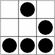
\includegraphics[width=0.5cm]{img/logo_glider.png} }
% \fancyfoot[RO]{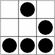
\includegraphics[width=0.5cm]{img/logo_glider.png} \hfill
	% TITLE
% \hfill \thepage /\pageref{LastPage}}
% \renewcommand{\headrulewidth}{0.5pt}
% \renewcommand{\footrulewidth}{0.5pt}
% \addtolength{\headheight}{0.5pt}
% \fancypagestyle{plain}{
	% \fancyhead{}
	% \renewcommand{\headrulewidth}{0pt}
% }

%--- Definitions de nouvelles commandes ---
\newcommand{\N}{\mathbb{N}} % les entiers naturels

%============================= Corps =================================
\begin{document}
\begin{landscape}

% \setcounter{page}{0}
% \thispagestyle{empty}

\begin{multicols}{2}

	\textsc{\Huge Memento LaTeX pour le JdR}~\\
	
	\tableofcontents
	
	\vfill
	\columnbreak
	
	\section{Idées de base}
	\begin{itemize}
		\item En-Tête, type de documents (livre, article, lettre...) ; 
		\item Comment compiler un document LaTeX ?
		\item Mise en page (par défaut, changements possibles, boites...) ;
		\item Table des matières : chapter, section, subsection, subsection... ; 
		\item Table des figures ; 
		\item Table de tableaux ; 
		\item Table des index et références ; 
		\item Insertions figures / images : ... ; 
		\item En-tête et Pied de page : types par défaut et personnalisation (fancyhdr) ; 
		\item Tableaux, Tableaux Longs ; 
		\item Tikz : décoration, frises, schémas, personnages, texte en travers, tikzpeople... ; 
		\item Polices de caractères / Fontes : usages, changements... ; 
		\item Beamer (faire des présentations)... ; 
	\end{itemize}
	
	\section{Rappel de règles de rédaction}
	
	\textbf{\textsc{Tu veux publier un document propre et clair ?~\\ Tu es au bon endroit !}}~\\
	
	Quelques rappels tout de même, que \LaTeX~ facilitera sans faire à ta place : 
	\begin{itemize}
		\item Accepte les relectures et corrections !
		\item L'orthographe et la grammaire sont importants (et essentiels), surtout pour que tes écrits persistent dans le temps et qu'ils puissent être facilement relus par d'autres (y compris le <<toi du futur>>) ;~\newline
			$\rightarrow$ Fait-toi relire (à défaut d'un correcteur orthographique correct) !!
		\item Concernant le style d'écriture : tant que tu trouves un public pour te lire et apprécier ton contenu, tout ira bien (sinon, il faut en changer). 
	\end{itemize}

	\vfill~\\
	\columnbreak
	
	\section{Introduction à \LaTeX}
	
	\subsection{Ce que permet \LaTeX}
	
	\begin{itemize}
		\item Offre une configuration par défaut et une mise en page conforme aux normes et standards de lisibilité et d'impression par défaut ; 
		\item Faire un minimum de mise en page sans trop réfléchir au départ (taille des caractères, police de caractère / fonte, justification du texte / égalisation sur les côtés par défaut...
		\item Des éléments de mise en page qui maintiennent la lisibilité en étant inclus dans celui-ci. 
		\item Utiliser des documents en texte brut (avec un logiciel du type de NotePad++, TextEditor, VIm, Nano, Emacs, Geany, Gedit, Jedit...) : 
		\begin{itemize}
			\item Utilise moins de place sur le disque dur ; 
			\item Compatible avec n'importe quel éditeur sur n'importe quel système ; 
			\item Éditable en WYSIWIG avec LyX ; 
			\item De la documentation et une communauté disponible en ligne (ou offline) et éprouvée ; 
			\item ...
		\end{itemize}
	\end{itemize}

	\subsection{Ce que NE permet PAS \LaTeX}
	
	\begin{itemize}
		\item Écrire à ta place. 
		\item Avoir un texte correct pour la grammaire et l'orthographe. 
		\item Avoir un style correct / lisible. 
		\item Avoir des idées à ta place (et empêcher d'en avoir). 
		\item ...
	\end{itemize}
	
	\vfill~\\
	\columnbreak
	
	\section{Bases : En-Tête, type de documents (livre, lettre...)}
	\section{Comment compiler un document LaTeX ?}
	\section{Mise en page (par défaut, changements possibles, boites...)} 
	\section{Table des matières : part, chapter, section, subsection, subsection...} 
	\section{Table des figures} 
	\section{Table de tableaux} 
	\section{Table des index et références} 
	\section{Insertions figures / images}  
	\section{En-tête et Pied de page : types par défaut et personnalisation (fancyhdr)} 
	\section{Tableaux, Tableaux Longs} 
	\section{Tikz : décoration, frises, schémas, personnages, texte en travers, tikzpeople...}  
	\section{Polices de caractères / Fontes : usages, changements...} 
	\section{Beamer (faire des présentations)...}
	
	...
\end{multicols}

\clearpage

\end{landscape}
\end{document}
